\section{System Overview}
\label{sec:overview}

The Debug System is designed to let a debugger feed a halted hart arbitrary
instructions, while keeping gate count to a minimum. This is necessary
functionality, and once it exists it can be used to accomplish all debug tasks.
To speed up certain repetitive operations, an optional Instruction Buffer can
be implemented. This is designed so that debug software can easily take
advantage of it, without needing a separate implementation for when it is and
isn't supported.

Figure~\ref{fig:overview} shows the main components of External Debug Support.
Blocks shown in dotted lines are optional.

\begin{figure}
   \centering
   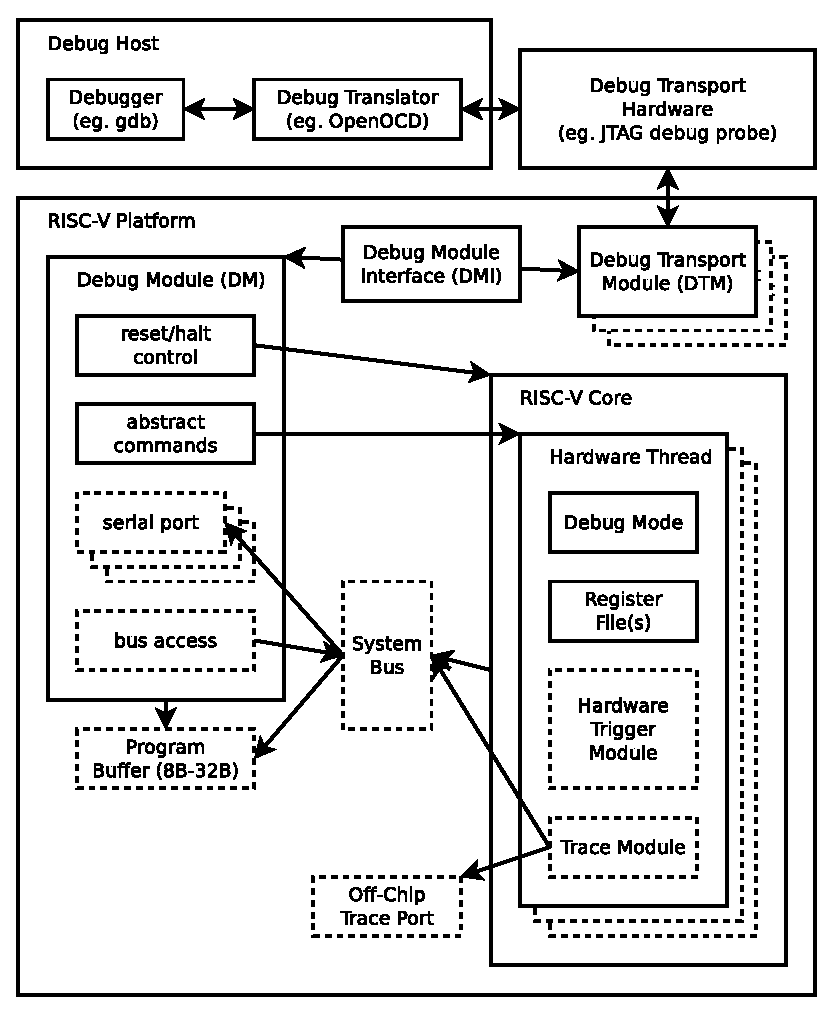
\includegraphics[width=\textwidth]{overview.eps}
   \caption{RISC-V Debug System Overview}
   \label{fig:overview}
\end{figure}

The user interacts with the Debug Host (eg. laptop), which is running a
debugger (eg. gdb).  The debugger communicates with a Debug Translator (eg.
OpenOCD, which may include a hardware driver) to communicate with Debug
Transport Hardware (eg.  Olimex USB-JTAG adapter) that's connected to the host.
The Debug Transport Hardware connects the Debug Host to the Platform's Debug
Transport Module (DTM).  The DTM provides access to the DM using the Debug
Module Interface (DMI).

The DM allows the debugger to halt any hart in the platform.  When a hart is
halted the DM can cause it to execute arbitrary instructions, and the hart can
move data to/from the DM as well.  Optionally the DM can contain an Instruction
Buffer to feed instructions more efficiently. As a further extension a Scratch
RAM may be implemented which can be used to briefly halt a hart and execute a
few instructions without requiring any debugger interaction once the process
has started.

Each RISC-V core may implement a Trigger Module for each hart.  These can
implement breakpoints, which cause a hart to halt spontaneously.  When that
happens the DM notices because the hart will signal the DM that it's ready for
an instruction.
